%*************************************************
\section{Cross-correlation in DBaaS warehouse}
\label{DBaaSCrossCorrelationSection}
%*************************************************
In Section \ref{LeakagePreventionSection} we defined a metric to evaluate exact value of information leakage due to attribute cross-correlation. However, a search algorithm to discover all of the cross-correlations among $m$ databases, each including $n$ documents, requires a search on an exponentially increasing space which is almost unfeasible computationally. The growth rate of cross-correlation analysis of $m$ databases necessitates examining all of the possible combinations of all databases which is computationally impractical. Therefore, in this Section, we propose a approach to approximate the cross-correlation amount between multiple databases. 

One of the limitations of random sample-based AQP schemes is their inaccurate approximation for a join aggregation queries that involve multiple databases with correlated attributes. Figure \ref{fig:cross-correlationMap} illustrates the cross-correlations between four example databases. 

\begin{figure}[H]
\centering
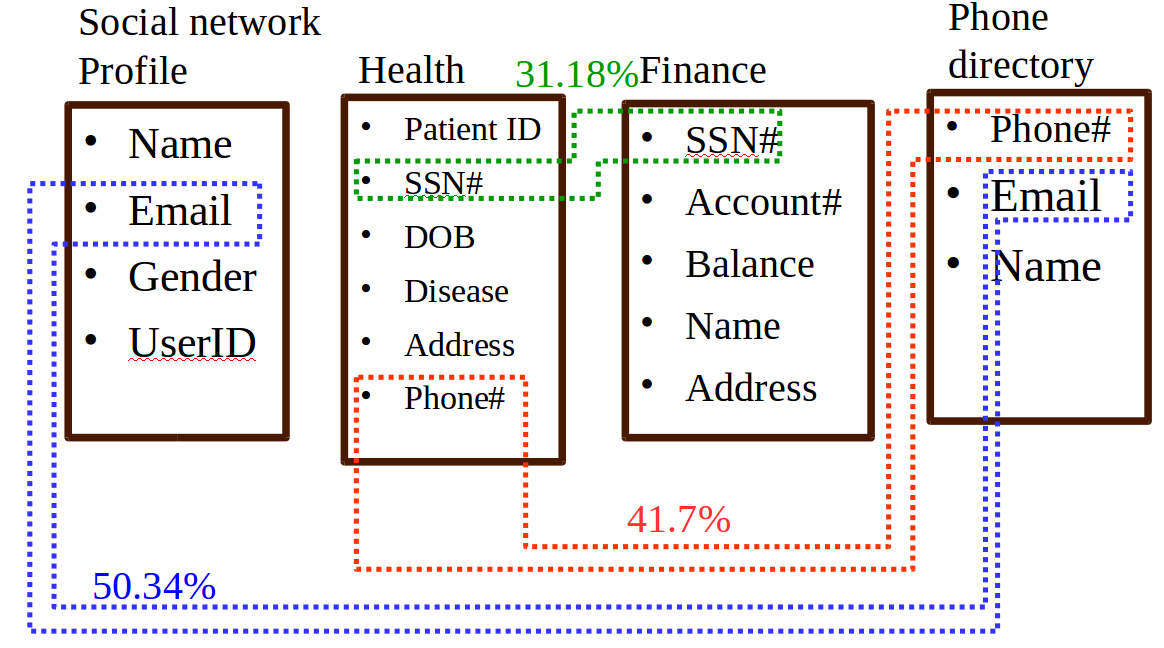
\includegraphics[width=0.7\linewidth]{figures/cross-correlationMap}
\caption[Cross-correlation map]{Four datasets containing $10^7$ documents with specific amount of cross-correlation are used in the estimation algorithm.}
\label{fig:cross-correlationMap}
\end{figure}

In order to attenuate the aforementioned problems, (computationally unfeasible  and inaccurate approximation), biased sampling method is considered to  provide more accurate responses for join aggregate queries. In such a scenario, extra information will be used for sampling from the base collections to preserve their relationships in the resulting sample set. The goal of this section is to use the extra information to produce biased sampling instead of random one. The class of documents with higher sensitivity ranking, the more possibility to be selected in the biased sample. In fact applying additional information (other attributes from the collection) in biased sampling phase facilitates cross-correlations discovering in the next phase. The biased sampling method only targets the highly sensitive attributes or the class of the interested documents selected from the database to form sample set. Although, biased sampling can be relatively pessimistic method, but since it focuses only on the crucial group of documents, the approximated answers are much closer to the exact answers. For example, consider two databases of secret devices and sensitive components, among which the correlation is supposed to be extracted. First, an AQP-based sensitivity analysis is performed on both collections to identify the most sensitive class in each database. Next, the biased samples are selected from these sensitive classes. The the proposed method has two phases, first, identifying correlated keys, second, approximating the size (cardinality) of cross-correlation using AQP approach.


\noindent \textbf{Correlated keys identification with AQP:} The idea is to first create a graph of documents using the biased samples. In the graph, there is an edge between vertex $i$ to vertex $j$ if they both have the same identifier attribute (such as phone number, social security number, patient ID, ... ). Finding connected components in an undirected graph which can be done with well-known graph search algorithms\footnote{Such as Depth First Search(DFS) or Breadth First Search (BFS) algorithms} starting from every unvisited vertex. Moreover, in the resulted graph the nodes with higher degree demonstrates attributes that cause more cross-correlation. The sorted list of vertices based on their degree exposes the attributes that cause more cross-correlation in pool of the cloud databases. The time complexity of this analysis is $O\big( \binom{m}{2}.n^2 \big)$, where $m$ is the number of samples and $n$ is the number of documents in each sample.

\noindent \textbf{ Cross-correlation analysis:} Analysis of information leakage, as a result of existence of \emph{unintentional cross-correlations} among many terabyte or petabyte level datasets, outsourced in the cloud DBaaS is a very hard problem with exponential growth rate. To overcome this problem, we adopt the approximation technique based on the correlated sampling to provide fast approximation with an acceptable error. This method is based on analyzing very small samples, and discovering potential relationships with other datasets. Consequently, a quick estimation of cross-correlation as clear indicator for information leakage will be achievable. The introduced approximation method eliminates the need for extensive analysis of the original datasets for cross-correlation discovery.

Consider two collections, $C_i, C_j$, let $\complement_{ij}$ be the exact cross-correlation between these collections. Cardinality of $\vert\complement_{ij}\vert$ presents the number of documents in $C_i$ and $C_j$ that have the same value for the correlation attribute. The subsequent subsections describe the cross-correlation size estimation method. 

%*************************************************
\subsection{Cross-correlation size estimation}
\label{correlatedEstimationSubSection}
%*************************************************

A set of random subset selected from the original collection which comprises of sensitive documents is constructed by uniform random sampling method. The selectivity probability $p_i$ for each sample $S_i$ is defined as $p_i=\frac{\vert S_i\vert}{\vert C_{i}\vert}$. In this method, first we apply AQP classification algorithm (discussed in the AQP classification section), to limit the cross-correlation analysis only to the much smaller space. In fact, with this approach, $\bowtie$ operator denoted as equality join is employed to measure the cardinality of cross-correlation between a uniform random sample $S_i$ joined to the biased sample. 

Suppose that, random sample sets are selected from users' profile database in a social media and phone directory which is limited to a particular demographic region of our interest. The average correlation size of those samples is a good approximation for true cardinality of correlation between the social media and phone directory. To deduce the estimated cross-correlation $\hat{\complement_{ij}}$,  Equation \ref{equ:CCEstimation} is used.

For instance, the average correlation size of random sample sets from users' profile database in a social media and phone directory which is limited to a particular demographic region is a good approximation for true cardinality of correlation between the that social media and phone directory. To deduce the estimated cross-correlation $\hat{\complement_{ij}}$ which is rephrased in Equation \ref{equ:CCEstimation}.

\begin{equation} 
\label{equ:CCEstimation}
\begin{aligned}
\vert \hat{\complement_{ij}}\vert=& \vert \complement^{\prime}_{ij}\vert \frac{1}{\min(p_i,p_j)}\\
\vert \hat{\complement_{ij}}\vert \approx & \vert \complement_{ij}\vert
\end{aligned}
\end{equation}
Where $\complement^{\prime}_{ij}$ is the cross-correlation between random sample $S_i$ and biased sample $S_j$ with selectivity probability of $p_i, p_j$ respectively.

%*************************************************
\subsection{Performance evaluation and experiments}
\label{PerformanceSubSection}
%*************************************************
We have a set of four datasets, including social network profile, health records, finance and phone directory each with $10^7$ documents. There are intentional cross-correlation between those datasets illustrated in Figure \ref{fig:cross-correlationMap}. The pipeline in the aggregate query is utilized to create equality join operator $\bowtie$ to extract documents from both given source and destination collections that match on the value of correlated attribute. The cross-correlation extractor query is displayed in Figure \ref{fig:CCQuery}. We applied the proposed estimation method to the sample sets with two different sizes and result is displayed in Figures \ref{fig:CCAproximation}. As it can be seen from figure, the bigger samples result in more accurate estimation. 

%Figure 
\begin{figure}[H]
\begin{framed}
{\ttfamily \small{ 
\textbf{db[source].aggregate}([\\\{\textbf{\$lookup :}\{\\\textbf{from :}destination,\\    \textbf{localField :}value,\\    \textbf{foreignField :}value,\\    \textbf{as :}"correlation" \}\},\\ \{\textbf{\$match :}\{"correlation":\{\textbf{\$ne :}[]\}\}\},\\
\{ \textbf{\$out :} saveToCollection \}\\]);
}
}
\end{framed}
\caption{Aggregate query for analysis of pairwise cross-correlation between two given source and destination collection.}
\label{fig:CCQuery}
\end{figure}


\begin{figure}[H]
\begin{subfigure}{0.5\textwidth}
\centering
\resizebox{1.0\textwidth}{!}{\begin{tikzpicture}[scale=1.0,trim axis right, trim axis right]
\begin{axis}[
compat=newest, 
legend style={at={(0.02,0.97)},anchor=north west},
ybar,
enlargelimits=0.12,
height=10cm,width=16cm,
bar width=20pt,
ylabel={Cross-correlation size},
symbolic x coords={{Health-Finance},{Social-Phone},{Phone-Health}},
xtick=data,
nodes near coords align={vertical}
,grid=major
,cycle list = {white,black!10,black!40,black!10,black!10}
]

\addplot+[fill=gray!80,text=black, draw=black, area legend,error bars/.cd,
y dir=both,y explicit] coordinates { %10000 documents
({Health-Finance},3123300)
({Phone-Health},5031080) 
({Social-Phone},4281100)
};
\addplot+[fill,text=black,  area legend,draw=black,pattern=north east lines,error bars/.cd, y dir=both,y explicit] coordinates { %100000 documents
({Health-Finance},3115910)
({Phone-Health},5036000) 
({Social-Phone},4265620)
};
\addplot+[fill,text=black, draw=black,  area legend,postaction={pattern=crosshatch},error bars/.cd, y dir=both,y explicit] coordinates { %Original correlation
({Health-Finance},3117847)
({Phone-Health},5033764) 
({Social-Phone},4170712)
};
\legend{Sample size $10^4$, Sample size $10^5$,Actual cross-correlations}
\end{axis}
\end{tikzpicture}
%\caption{}
%\label{fig:CCEstimation}}
\label{fig:CCEstimation}
\caption{}
\end{subfigure}
\qquad 
\begin{subfigure}{0.5\textwidth}
\resizebox{1.0\textwidth}{!}{\begin{tikzpicture}[scale=1.0,trim axis right, trim axis right]
\begin{axis}[
compat=newest, 
legend style={at={(0.02,0.97)},anchor=north west},
ybar,
enlargelimits=0.12,
height=10cm,width=16cm,
bar width=20pt,
ylabel={Error Percentage},
symbolic x coords={{Health-Finance},{Social-Phone},{Phone-Health}},
xtick=data,
nodes near coords align={vertical}
,grid=major
,cycle list = {white,black!10,black!40,black!10,black!10}
]
\addplot+[fill=gray!80,text=black, area legend, draw=black,error bars/.cd,
y dir=both,y explicit] coordinates { %10000 documents
({Health-Finance},0.6)
({Phone-Health},0.3) 
({Social-Phone},1.1)
};
\addplot+[fill,text=black,  area legend,draw=black,pattern=north east lines,error bars/.cd, y dir=both,y explicit] coordinates { %100000 documents
({Health-Finance},0.02)
({Phone-Health},0.02) 
({Social-Phone},0.95)
};
\legend{Sample size $10^4$, Sample size $10^5$}
\end{axis}
\end{tikzpicture}
}
\label{fig:speedup}
\caption{}
\end{subfigure}
\caption{The cardinality of cross-correlation estimation using two sets of samples with $10000$ and $100000$ documents: (a) Estimated values for the two sample sets, compared to the actual cross-correlation. (b) The estimation error percentage.}
\label{fig:CCAproximation}
\end{figure}